\documentclass{article}
\usepackage{graphicx}
\graphicspath{D:/Texmaker/graphics/images/}

\begin{document}
\title {including graphics}




\section{Introduction}
%\centering
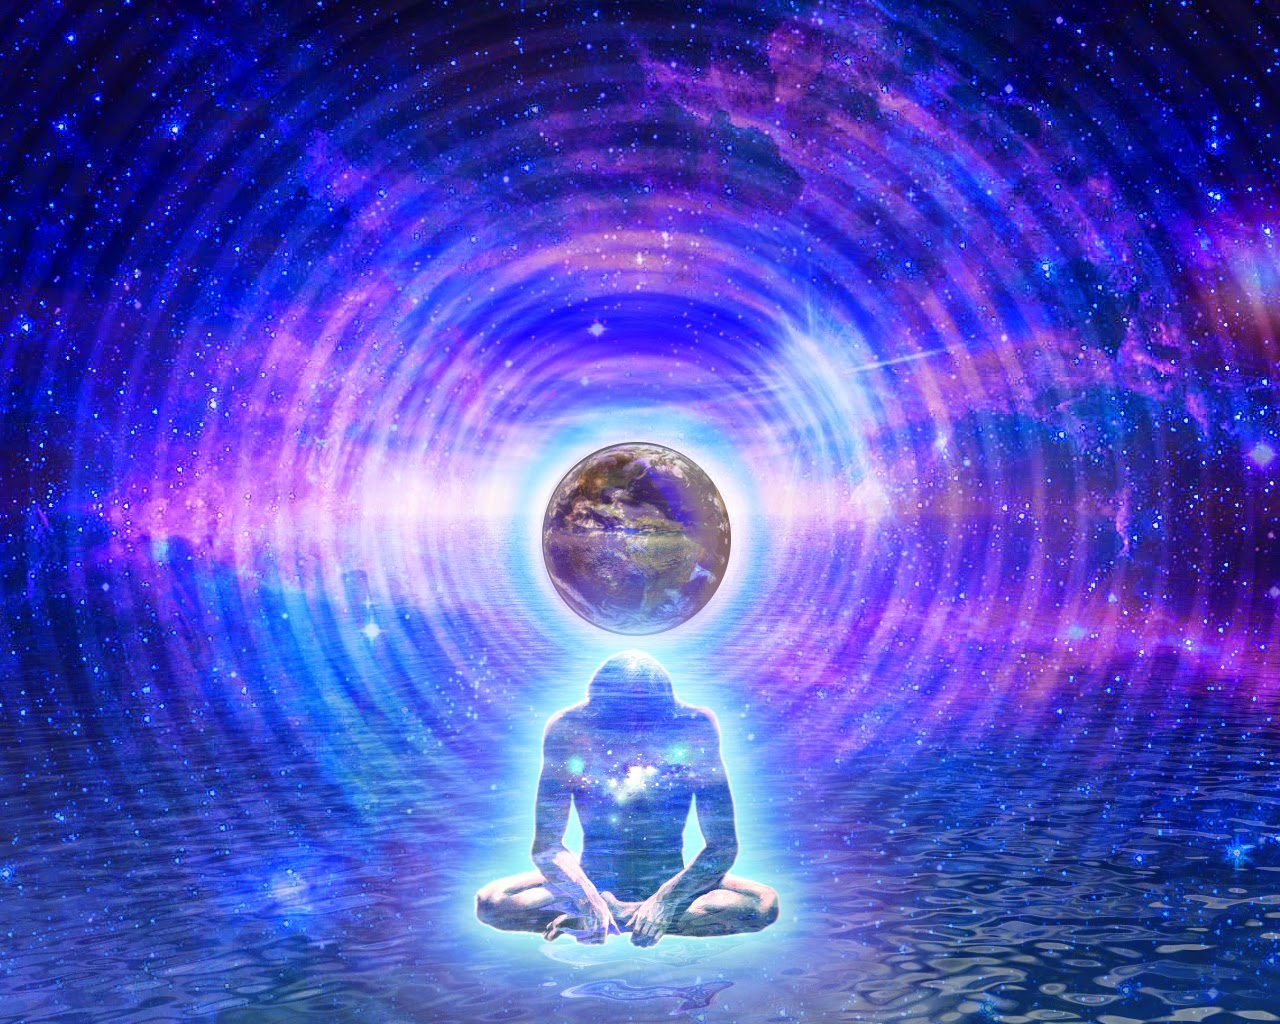
\includegraphics[width=3 in]{D:/Texmaker/graphics/images/meditate.jpg}






\subsection{Floating Figure Environment}


About 350,000 species of plants, defined as seed plants, bryophytes, ferns and fern allies, have been estimated to exist.

As of 2004, some 287,655 species had been identified, of which 258,650 are flowering and 15,000 bryophytes.

Plants are mostly autotrophs, organisms that obtain energy from sunlight or organisms that make their own food.

Most plants carry out a process called photosynthesis, which occurs in the chloroplasts of plants.
It is a common misconception that most of the solid material in a plant is taken from the soil, when in fact almost all of it is actually taken from the atmosphere.

In my article , I am going to use jpg image in floating env. in Figure\ref{fig:plant}


\begin{figure}
% for centering env.
\begin{center}
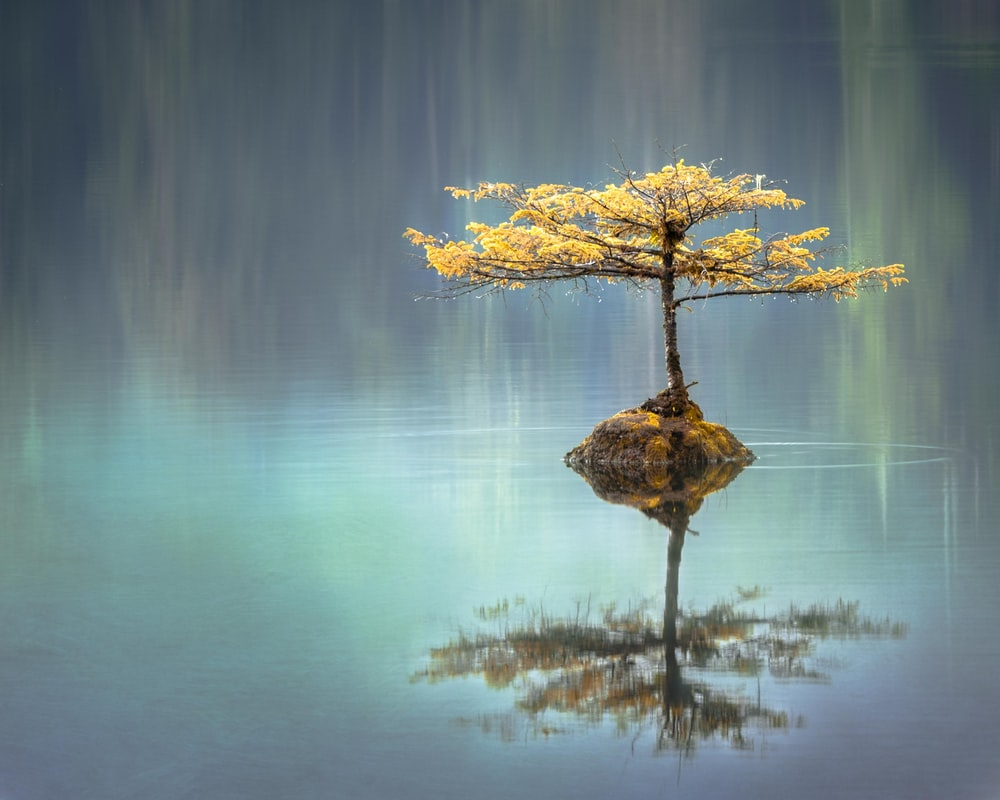
\includegraphics[width=3 in]{D:/Texmaker/graphics/images/plant.jpg}
\caption{Plant}
\label{fig:plant}
\end{center}
\end{figure}

\end{document}